\documentclass[a4paper,12pt]{article}

\usepackage[utf8]{inputenc}
\usepackage[slovene]{babel}
\usepackage{amsmath}
\usepackage{amsfonts}
\usepackage{relsize}
\usepackage[smaller]{acronym}
\usepackage{graphicx}
\usepackage{subfigure}
\usepackage{cite}
\usepackage{url}
\usepackage[unicode=true]{hyperref}
\usepackage{color}
\usepackage[version=3]{mhchem}
\usepackage{wrapfig}
\usepackage{comment}
\usepackage[left=2.5cm,right=2.5cm,top=2.5cm,bottom=2.5cm]{geometry}


%opening
\title{Hidrodinamske nestabilnosti v tankih plasteh}

\renewcommand{\vec}{\mathbf}
\newcommand{\eps}{\varepsilon}
% \renewcommand{\phi}{\varphi}
\renewcommand{\theta}{\vartheta}
\newcommand{\dd}{\,\mathrm{d}}

\newcommand{\odv}[1]{\frac{\partial #1}{\partial t}}

\newcommand{\norm}[1]{\lVert #1 \rVert}

\newcommand{\rt}{(\vec r, t)}

\begin{document}
\begin{center}

\includegraphics[width=6cm]{../logo_fmf_uni-lj_sl}\\[0.5cm]
Oddelek za fiziko \\[2cm]
{ \large Seminar -- 1. letnik, II. stopnja } \\[1cm]
{ \huge \bf Hidrodinamske nestabilnosti \\ v tankih plasteh}\\[2cm]
{\large Avtor: Miha \v Can\v cula}\\[0.6cm]
{\large Mentor: prof. dr. Alojz Kodre} \\[0.6cm]
{\large Ljubljana, marec 2012}
\end{center}
\vfill

\begin{abstract}

V hidrodinamiki lahko najdemo razli"cne pojave, kjer je tok teko"cine nestabilen. Nekateri izmed teh pojavov nastopajo pri gibanju teko"cine v tanki plasti, kjer lahko za poenostavitev ena"cb uporabimo lubrikacijski pribli"zek. Primere lahko najdemo v vsakdanjem "zivljenju, na primer tok teko"cine po nagnjeni povr"sini ali razpad opne milni"cnega mehur"cka. Z uporabo primernih ra"cunskim modelov lahko napovemo stabilnost tak"snih sistemov. 


\end{abstract}

\newpage

\tableofcontents

\section{Uvod}

O nestabilnosti govorimo, ko infinitezimalno majhna sprememba trenutnega stanja lahko povzro"ci ve"cjo, merljivo razliko po nekem kon"cnem "casu~\cite{drazin}. Na nestabilnosti naletimo na mnogih podro"cjih fizike. Zaradi zapletenosti ena"cb in izobilja razli"cnih pogojev so "se posebej zanimive tiste, ki izhajajo iz "studija gibanja teko"cin, hidrodinamike. 

Hidrodinamika je zelo "siroko podro"cje, ena"cbe, ki opisujejo gibanje teko"cin, pa zahtevne za re"sevanje, zato se poslu"zimo dolo"cenih poenostavitev in pribli"zkov. V tem seminarju sem se posvetil le tankim plastem teko"cine. Na ta na"cin si lahko ena"cbe poenostavimo do tak"sne mere, da jih bomo znali re"siti vsaj numeri"cno, vseeno pa tudi v tako zmanj"sanem naboru sistemov najdemo veliko zanimivih problemov. Vse obravnavane primere tudi dobro poznamo iz vsakdanjega "zivljenja. 

\section{Stabilnost in zlom simetrije}

Zgornja definicija nestabilnosti je precej splo"sna, zato jo za potrebe seminarja raje definiramo o"zje in bolj eksaktno. Stabilnost sistema pomeni, da vse motnje, ki so na za"cetku majhne, ostanejo majhne tudi ob poljubnem "casu. Nasprotno, sistem je nestabilen, "ce vsaj ena motnja po nekem "casu preneha biti majhna. Obi"cajno to pomeni, da za vsako motnjo, ki je ob za"cetnem "casu omejena z neko zgornjo mejo, obstaja neka druga zgornja meja, ki je motnja nikoli ne prese"ze. 

"Ce se poleg stabilnosti motnja s "casom manj"sa, je tok \emph{asimptoti"cno stabilen}. V teoriji dinami"cnih sistemov asimptoti"cno stabilni re"sitvi re"cemo tudi atraktor. 

Stabilnost oz. nestabilnost sistema je tesno povezana z zlomom simetrije. Predstavljajmo si sistem, katerega "casovno spreminjanje lahko opi"semo z eno ali ve"c diferencialnimi ena"cbami, ki imajo dolo"ceno simetrijo. Z nastavkom, ki upo"steva to simetrijo, dobimo re"sitev ena"cb. Stabilnost se poka"ze, ko temu nastavku dodamo majhno motnjo, ki ne upo"steva simetrije. Stabilni sistem se bo vrnil v simetri"cno stanje, medtem ko pri nestabilnem pride do zloma simetrije. 

Primer nestabilnega pojava je svin"cnik, postavljen na konico. Ena"cba, ki opisuje njegovo gibanje, je simetri"cna glede na rotacijo okrog osi svin"cnika. Zato lahko najdemo re"sitev z enako simetrijo, to je pokon"cna lega. "Ce pa svin"cnih le malo izmaknemo iz simetri"cne lege, bo padel v dolo"ceno smer in kon"cal v stanju brez rotacijske simetrije. 

Po drugi strani pa je te"zno nihalo stabilen sistem. "Ce tak"sno nihalo zmotimo, bo motnja vseskozi ostajala pribli"zno enake velikosti, zaradi trenja in zra"cnega upora se bo s "casom celo manj"sala. Po dolgem "casu bo sistem spet v simetri"cnem stanju. 

\section{Hidrodinamika}

\subsection{Navier-Stokesova ena"cba}

Tok nestisljive teko"cine z gostoto $\rho$ in viskoznostjo $\mu$ se podreja Navier-Stokesovi ena"cbi in ohranitvi mase. Ena"cbi za hitrost $\vec u\rt$ in tlak $p\rt$ se glasita

\begin{align}
 \label{eq:ns-enacba}
\frac{\partial \vec u}{\partial t} + (\vec u \cdot \nabla) \vec u &= -\frac{1}{\rho}\nabla p + \mu \Delta \vec u \\
\nabla \vec u &= 0
\end{align}

kjer je $\rho$ gostota teko"cine, $\mu$ pa njena viskoznost. 

Ena"cbi lahko poenostavimo s prehodom na brezdimenzijske spremenljivke in s tem zmanj"samo "stevilo parametrov. Izberimo si meri za dol"zino $x_0$ in hitrost $v_0$. "Ce uvedemo "se brezdimenzijsko Reynoldsovo "stevilo $R=v_0 x_0 / \mu$, lahko za brezdimenzijski spremenljivki $\vec U$ in $P$ zapi"semo

\begin{align}
 \label{eq:ns-brezdim}
\frac{\partial \vec U}{\partial t} + (\vec U \cdot \nabla) \vec U &= -\nabla P + R^{-1} \Delta \vec U \\
\nabla \vec U &= 0
\end{align}

V sistemu ena"cb nastopa le en prost parameter. Poleg tega parametra je re"sitev ena"cbe odvisna "se od za"cetnih in robnih pogojev. Obi"cajno poznamo za"cetni profil hitrosti in tlaka, saj si ju lahko izberemo ali ju izmerimo s poskusom. Robni pogoji v razli"cnih geometrijah pa so lahko zelo zapleteni in mo"cno ote"zijo ra"cunanje. 

\subsection{Lineariziran problem}

Stabilnost hidrodinamskega sistema lahko "studiramo tako, da najprej najdemo osnovno re"sitev, ki ji v hidrodinamiki re"cemo \emph{osnovni tok}. Ta re"sitev je lahko podana analiti"cno ali numeri"cno, vsekakor pa se podreja Navier-Stokesovi ena"cbi. 

Nato osnovnem toku dodamo motnjo, tako da dobimo \emph{skupni tok}, zopet podan s hitrostjo $\vec u = \vec U + \vec u'$ in tlakom $p = P + p'$. Tudi za skupni tok mora veljati N-S ena"cba, iz "cesar lahko izpeljemo ena"cbo za motnjo $u'$ in $p'$. 

Ker nas zanimajo le majhne motnje, lahko v ena"cbi zanemarimo vse "clene, kjer motnja nastopa v drugem ali vi"sjih redih. Na ta na"cin sistem zreduciramo nov na sistem linearnih diferecialnih ena"cb 

\begin{align}
 \label{eq:ns-linearna}
\frac{\partial \vec u'}{\partial t} + (\vec U \cdot \nabla) \vec u' + \vec u' \cdot \nabla \vec U &= -\nabla p' + R^{-1}\Delta u' \\
\label{eq:nestisljivost-linearna}
\nabla \cdot \vec u' &= 0
\end{align}

"Ce je osnovni tok stacionaren, so koeficienti v linearnem sistemu ena"cb konstantni, torej tak"sen sistem znamo re"siti. Lo"cimo lahko spremenljivki $\vec r$ in $t$, splo"sno re"sitev pa zapi"semo kot linearno kombinacijo

\begin{align}
 \vec u'\rt &= \sum e^{s_i t} \vec u_i(\vec r) \\
 p'\rt &= \sum e^{s_i t} p_i(\vec r)
\end{align}

kjer so $\vec u_i$ in $p_i$ lastni valovni na"cini. Ker sta ena"cbi linearni v kraju, je njihova krajevna odvisnost harmoni"cna. 

Hitro vidimo, da bo tok nestabilen, "ce ima vsaj ena lastna vrednost $s_i$ realni del ve"cji od 0, v nasprotnem primeru pa bo stabilen. Problem stabilnosti sistema lahko torej prevedemo na re"sevanje sistema linearnih ena"cb, kar je enakovredno iskanju lastnih vrednosti matrike. Sedaj tudi vidimo, da matemati"cno natan"cni definiciji mere za velikost motnje in kriterija za stabilnosti nimata velikega pomena, saj motnje v obliki normalnih valovnih na"cinov le eksponentno nara"s"cajo ali padajo, njihova oblika pa ostaja enaka. 

Tak"sna poenostavitev velja le za majhne motnje. "Ce je sistem nestabilen in se motnja s "casom pove"ca, bo po nekem "casu presegla mejo, kjer je lineariziran pribli"zek "se smiselen. Tedaj moramo v ena"cbi upo"stevati tudi vi"sje "clene, zato le-ta ni ve"c linearna. 

\subsection{Lubrikacijski pribli"zek}

V geometrijah, kjer je ena izmed dimenzij mnogo manj"sa od ostalih, si lahko gibalne ena"cbe poenostavimo z lubrikacijskim pribli"zkom (angl. lubrication approximation). Odvisnost od te koordinate lahko izlo"cimo in s tem zmanj"samo "stevilo spremenljivk v Navier-Stokesovi ena"cbi. 

Na tanki plasti teko"cine obstajata dve razlicni dol"zinski skali, od katerih so odvisni velikostni redi nekaterih spremenljivk. Izberimo si koordinatni sistem, kjer je os $z$ v smeri najmanj"se dimenzije. Poljubna sprememba koordinate $z$ bo vedno dosti manj"sa od primerljive spremembe v ravnini, iz "cesar lahko zaklju"cimo 

\begin{enumerate}
  \item Komponenta hitrosti v smeri $z$ je dosti manj"sa od komponent v smereh $x$ in $y$. 
  \item Odvod poljubne spremenljivke po $z$ je dosti ve"cji od odvoda v ravnini. 
\end{enumerate}

Pri ra"cunih lahko nekatere izmed "clenov v Navier-Stokesovih ena"cbah zanemarimo. Ker pa imamo sedaj smer, v kateri se teko"cina obna"sa druga"ce kot v ostalih, imamo namesto ene vektor"ske ena"cbe razli"cni ena"cbi v smereh $z$ in $xy$. V definiciji Reynoldsovega "stevila nastopa tudi velikostna skala, ki je v tanki plasti enaka debelini plasti, torej majhni dimenziji, $R = v_0 z_0/\mu$. V tak"sni geometriji lahko vedno ra"cunamo v limiti, ko je Reynoldsovo "stevilo majhno. 

Poleg izpu"s"canja "clenov v ena"cbi pa nam tanka plast teko"cine omogo"ca "se eno spremembo. "Ce nas odvisnost hitrosti od vi"sine $z$ ne zanima, lahko hitrost povpre"cimo po debelini filma

\begin{align}
 \vec u(x,y) &=  \frac{1}{h}\int_0^h \vec u(x,y,z)\dd z
\end{align}

kjer je $h = h(x,y)$ debelina plasti na mestu $(x,y)$. Ohranitev mase da zvezo med $h$ in $\vec u$

\begin{align}
  \frac{\partial h}{\partial t} + \nabla\cdot(h\vec u) = 0
\end{align}

s "cimer lahko Navier-Stokesove ena"cbe zapi"semo za spremenljivko $h(x,y,t)$. Namesto "stirih skalarnih koli"cin $\vec u$ in $p$ v poenostavljeni ena"cbi nastopa le ena koli"cina, kar olaj"sa re"sevanje. S tem korakom seveda izgubimo del informacije o re"sitvi, saj iz re"sitve za $h$ ne moremo rekonstruirati hitrostnega profila v smeri $z$. Za ugotavljanje stabilnosti tanke plasti teko"cine pa je dovolj re"sevati ena"cbo z eno samo skalarno spremenljivko. 

\section{Teko"cina na klancu}

\begin{figure}[h]
\centering
 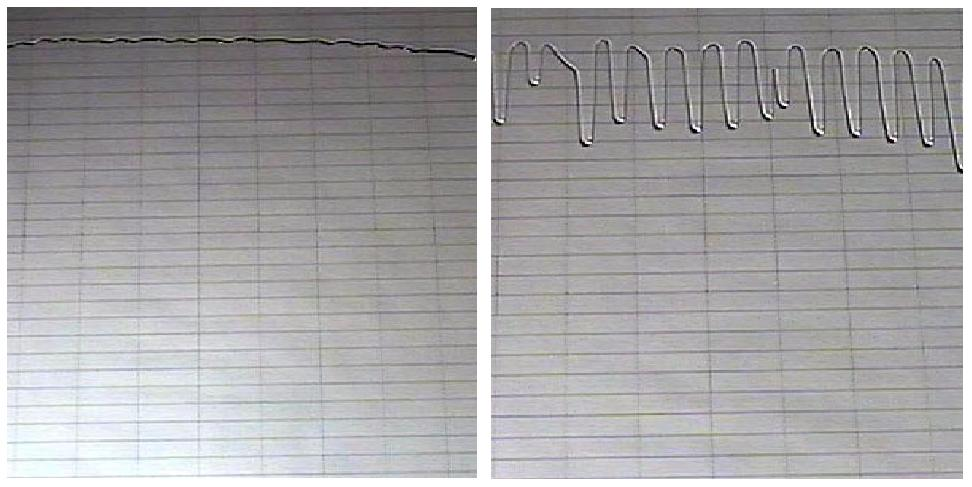
\includegraphics[width=.9\textwidth]{./Slike/film-slika}
\caption{Polzenje tanke plasti teko"cine po nagnjeni povr"sini. Majhne motnje v obliki fronte (levo) hitro prerastejo v vzorec, ki ni enakomeren, je pa pribli"zno periodi"cen (desno). Vir: \cite{kondic}}
\label{fig:film-neenakomernost}
\end{figure}

Hidrodinamsko nestabilnost lahko opazujemo pri polzenju teko"cine po klan"cini~\cite{kondic}. Ta pojav je vsem dobro znan, saj ga lahko vidimo na avtomobilskih steklih v de"zju, enostavno pa je tudi pripraviti poskus doma. "Ceprav je re"sevanje ena"cb zahteveno, lahko rezultat preverimo z eksperimentom. 

Vzorec na sliki~\ref{fig:film-neenakomernost} lahko pojasnimo s kratkim razmislekom. Po klan"cini navzdol vodo poganja sila te"ze, zadr"zujeta pa jo viskoznost in povr"sinska napetost, ki pa imata velik vpliv le na tanke plasti. "Ce majhna motnja ob nekem trenutku povzro"ci, da je na nekem mestu plast voda debelej"sa, imata tako viskoznost kot povr"sinska napetost manj"si vpliv na gibanje vode kot sila te"ze. Na tistem mestu steklo ve"c vode kot drugod, kar bo le okrepilo za"cetno motnjo, tako da bo na tistem mestu voda vedno la"zje tekla. 

Le z razmislekom pa ne znamo napovedati niti kon"cne oblike fronte niti povpre"cne razdalje med mesti z ve"cjim pretokom. "Ce nas to zanima, moramo tudi kaj izra"cunati. 

\subsection{Ena"cbe}

"Ce privzamemo nestisljivost teko"cine $\nabla \cdot \vec u = 0$, se Navier-Stokesova ena"cba za teko"cino na klancu glasi 

\begin{align}
 \label{eq:ns-film}
 \frac{\partial \vec u}{\partial t} + (\vec u \cdot \nabla) \vec u\ &= -\frac{1}{\rho}\nabla p + \frac{\mu}{\rho}\nabla^2 \vec u + g (\sin \alpha \vec i - \cos \alpha \vec k)
\end{align}

kjer je $\vec u$ hitrost teko"cine, $\rho$ njena gostota in $\mu$ viskoznost. "Clena z $g$ sta dinami"cna in stati"cna komponenta sile te"ze. Pomembni so tudi robni pogoji, obi"cajno se izbere slede"ce:

\begin{itemize}
 \item Na meji med teko"cino in klancem teko"cina ne drsi, torej je tam $\vec u = 0$. 
 \item Na meji med teko"cino in zrakom ima tlak nezveznost zaradi povr"sinske napetosti teko"cine. Nezveznost je sorazmerna s povr"sinsko napetostjo in ukrivljenostjo meje $\kappa$. 
\end{itemize}

Ker obravnavamo tanke filme, lahko privzamemo, da je debelina $h$ manj"sa od katerekoli dol"zinske skale v ravnini $xy$. Uporabimo lubrikacijski pribli"zek, ukrivljenost meje med teko"cino in zrakom pa ocenimo s $\kappa \approx \nabla^2 h$. S tem privzetkom lahko ena"cbo (\ref{eq:ns-film}) poenostavimo v ena"cbo za $h$. 

\begin{align}
\label{eq:ns-film-h}
 \frac{\partial h}{\partial t} = -\frac{1}{3\mu}\nabla \cdot \left[ \gamma h^3 \nabla \nabla^2 h - \rho g h^3 \nabla h \cos \alpha + \rho g h^3 \sin \alpha \vec i \right]
\end{align}

\begin{figure}[h]
\centering
 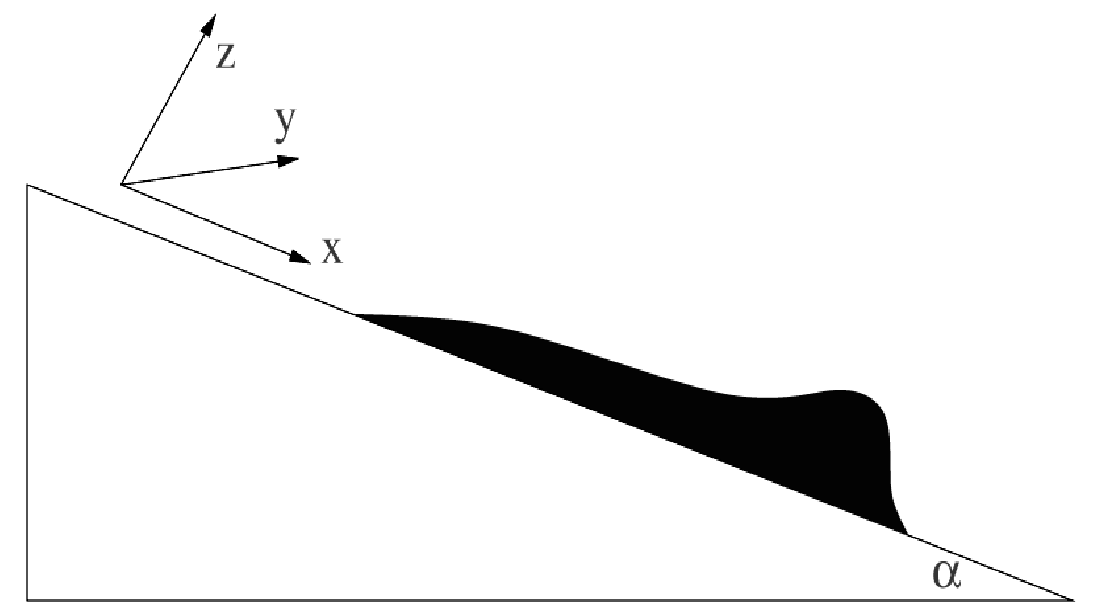
\includegraphics[width=.6\textwidth]{./Slike/film-skica}
\caption{Skica teko"cine na klancu v dveh dimenzijah. Viden je greben tik za fronto teko"cine in pa zo"zitev dale"c za fronto. Pri ra"cunih raje privzamemo, da teko"cina sproti priteka z zgornjega roba klan"cine, tako da zo"zitve ni treba upo"stevati}
\label{fig:film-skica}
\end{figure}

Zgornja ena"cba je simetri"cna glede na poljuben premik v kraju in "casu, saj te koli"cine v njej ne nastopajo eksplicitno. Za"cetno stanje, kot je prikazano na sliki~\ref{fig:film-skica} pa podaja odvisnost debeline plasti od $x$ in $z$. Iz postavitve problema sklepamo, da se bo "celo teko"cine s "casom premikalo po klancu navzdol, torej bo profil odvisen od "casa. Edina simetrija, ki ji zado"s"cata tako za"cetno stanje kot gibalna ena"cba je torej translacijska v smeri $y$. 

\begin{figure}[h]
 \centering
 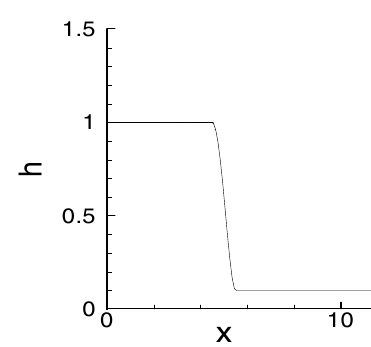
\includegraphics[width=.4\textwidth]{./Slike/film-zacetni}
 \caption{Za"cetni pogoj za dolo"canje toka teko"cine po klancu. }
 \label{fig:film-zacetni}
\end{figure}

Da najdemo osnovno re"sitev, najprej privzamemo, da ima re"sitev enako simetrijo kot sama ena"cba. Postavimo se v koordinatni sistem kot na sliki~\ref{fig:film-skica}. Klanec, po katerem te"ce teko"cina, ima translacijsko simetrijo v smeri $y$, zato za osnovno re"sitev velja $h_y = 0$. Za la"zje re"sevanje preidemo "se na brezdimenzijske koli"cine. V ena"cbi ostane le "se en parameter $D(\alpha)$, ki podaja razmerje med vplivom viskoznosti in povr"sinske napetosti, brezdimenzijsko dol"zino klanca v smeri $x$ pa ozna"cimo z $L$. Ena"cba za brezdimenzijske koli"cine, ki predpostavlja simetrijo in zato opisuje osnovno re"sitev problema, se glasi

\begin{align}
  \label{eq:ns-film-sim}
 \odv{h} &= - \left[h^3 h_{xxx}\right]_x + D(\alpha) \left[h^3 h_x\right]_x - \left(h^3\right)_x
\end{align}

Pred za"cetkom re"sevanja moramo dolo"citi tudi za"cetne in robne pogoje. Ena"cba je "cetrtega reda v $x$, zato potrebujemo "stiri robne pogoje in profil teko"cine ob "casu $t=0$. Za za"cetno stanje si izberimo profil, kot je na sliki~\ref{fig:film-zacetni}. Pri tak"sni izbiri velja $h(0, t) = 1$ po definiciji brezdimenzijske debeline, pred fronto pa je plast mnogo tanj"sa, $h(L, t) = b \ll 1$. Velikost domene $L$ mora biti ve"cja od razdalje, ki jo bo prepotovalo "celo teko"cine. Oba robna pogoja ne veljata le na robu obmo"cja, ampak tudi v njegovi bli"zini, zato za ostala dva robna pogoja vzamemo $h_x(0,t) = h_x(L,t) = 0$. 

Zgornja ena"cba je "se vedno prezahtevna, da bi jo re"sevali analiti"cno, zato pose"zemo po numeri"cnih metodah. Re"sitev ena"cbe (\ref{eq:ns-film-sim}) lahko dobimo z uporabo metode na osnovi kon"cnih diferenc. 

\begin{figure}[h]
 \centering
 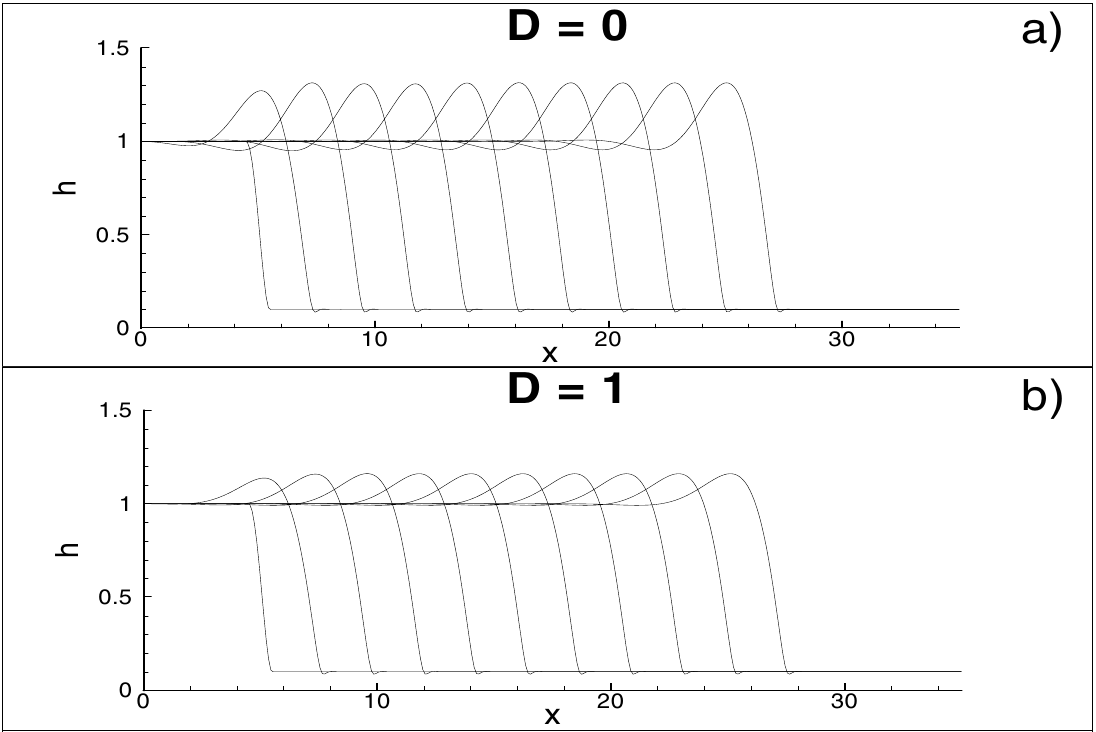
\includegraphics[width=.8\textwidth]{./Slike/film-osnovna-resitev}
 \caption{Profil teko"cine pri razli"cnih vrednostih parametra $D$. V obeh primerih se hitro oblikuje greben tik za fronto. Profili so prikazani v intervalih $\delta t = 2$, pri izbranih vrednostih $L = 40$ in $b=0,1$. Koordinata $x$ je diskretizirana s korakom $\Delta x = 0,05$~\cite{kondic}. }
 \label{fig:film-osnovna}
\end{figure}

\subsection{Nestabilnost}

Osnovna re"sitev $h_0(x, t)$ je sicer odvisna od "casa, vendar lahko predpostavimo, da "celo teko"cine polzi s konstantno hitrostjo $U$. "Casovno odvisnost koeficientov $h_0$ bomo torej odpravili, "ce se postavimo v koordinatni sistem, ki se giblje s to hitrostjo. V tem primeru uvedemo spremenljivko $\xi = x - Ut$, splo"sno re"sitev pa lahko zapi"semo v obliki

\begin{equation}
 h(\xi, y, t) = h_0(\xi) + \eps h_1(\xi, y, t)
\end{equation}

V tej sliki se $h_0$ ne spreminja s "casom, torej smo dobili linearno diferencialno ena"cbo s konstantnimi koeficienti. Ker "zelimo, da je motnja res majhna, predpostavimo, da sta $h_0$ in $h_1$ podobnega velikostnega reda, $\eps$ pa zelo majhen, mnogo manj"si od 1. Zgornji izraz vstavimo v ena"cbo (\ref{eq:ns-film-h}) in zanemarimo vse "clene z drugo in vi"sjimi potencami $\eps$. 

Motnjo $h_1$ izberemo tak"sno, da zanjo ne dr"zi translacijska simetrija v smeri $y$. Na sliki~\ref{fig:film-neenakomernost} vidimo, da je oblika fronte pribli"zno periodi"cna, zato poskusimo s harmoni"cno motnjo oblike $h_1(\xi, y, t) = g(\xi, t) \exp (i q y)$. Tak"sna motnja z valovnim "stevilo $q$ ima valovno dol"zino $\lambda = 2\pi/q$. Ker motnja zado"s"ca linearni ena"cbi, je njena "casovna odvisnost eksponentna

\begin{align}
  h_1(\xi, y, t) &= \phi(\xi) e^{iqy} e^{s t}
\end{align}

Tako $\phi$ kot $s$ sta odvisni od valovnega "stevila $q$. "Ce je realni del $s$ pozitivna, bo majhna motnja eksponentno nara"s"cala in povzro"cila zlom simetrije. Pri"cakujemo, da bo valovna dol"zina, pri kateri je vrednost $s$ najve"cja, enaka razdalji med posameznimi pasovi na sliki~\ref{fig:film-neenakomernost}, saj bo motnja s tak"sno valovno dol"zino najhitreje nara"s"cala. Odvisnost $s(q)$, izra"cunana numeri"cno, je prikazana na sliki~\ref{fig:film-rast}. Valovna dol"zina najhitrej"se rasti je odvisna od parametra $D$, prav tako pa tudi hitrost rasti in z njo karakteristi"cni "cas, po katerem motnja postane vidna. 

\begin{figure}[h]
 \centering
 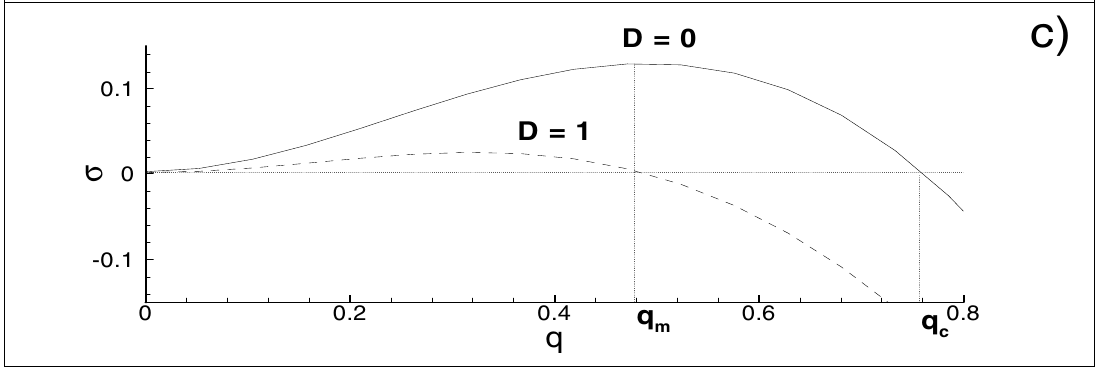
\includegraphics[width=.8\textwidth]{./Slike/film-stabilnost}
 \caption{Hitrost rasti $s$ majhne motnje z valovnim "stevilom $q$. Valovna dol"zina z najhitrej"so rastjo $\lambda_m = 2\pi/q_m$ ustreza pri"cakovani razdalji med curki.~\cite{kondic}. }
 \label{fig:film-rast}
\end{figure}

\newpage
\section{Milni mehur"cki}

\begin{figure}[h]
 \centering
\subfigure{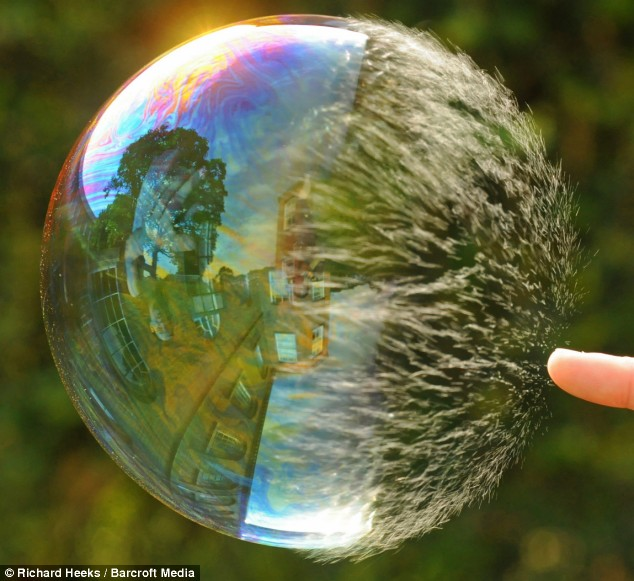
\includegraphics[height=.45\textwidth]{./Slike/bubble-3}}
\subfigure{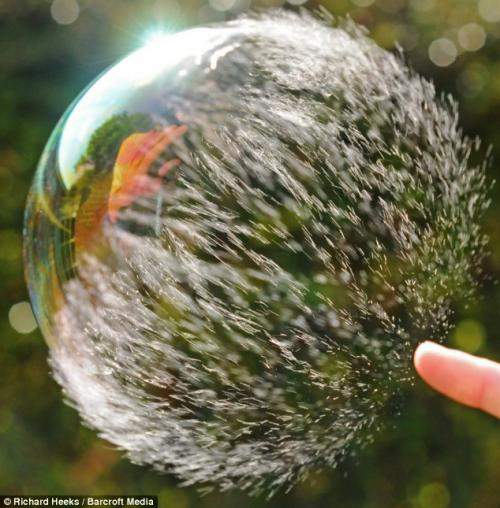
\includegraphics[height=.45\textwidth]{./Slike/bubble-4}}
\caption{Razpad milnega mehur"cka~\cite{slike-mehurcek}. }
\label{fig:mehurcek-3}
\end{figure}

Milni mehur"cki so stabilni, saj majhne motnje v opni zadu"si povr"sinska napetost teko"cine. "Ce pa mehur"cek predremo v eni to"cki, ustvarimo rob, kjer povr"sinska napetost ni uravnote"zena, zato se rob za"cne umikati. Ker je opna zelo tanka, je ukrivljenost na robu velika, zato fronta napreduje zelo hitro~\cite{diploma}. To napredovanje je pri mehur"ckih tako hitro, da s prostim o"cesom fronte sploh ne opazimo, ampak se nam zdi, da celoten mehur"cek razpade naenkrat. Pri opazovanju si lahko pomagamo s hitrimi kamerami, kot vidimo na sliki~\ref{fig:mehurcek-3}. 

Podobno kot pri tankem filmu tudi tu obravnavamo tanko plast teko"cine pod vplivom povr"sinske napetosti. Skica roba opne z ozna"cenimi spremenljivkami in koordinatnimi osmi je na sliki~\ref{fig:mehurcek-skica}. 
\begin{figure}[h]
 \centering
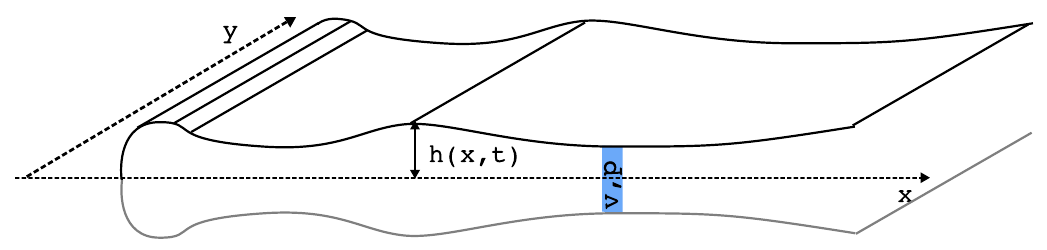
\includegraphics[width=.8\textwidth]{./Slike/mehurcek-skica}
\caption{Profil opne s translacijsko simetrijo vzdol"z roba in zrcalno simetrijo v navpi"cni smeri. Ker je opna tanka, lahko privzamemo, da se tlak in hitrost ne spreminjata po debelini~\cite{diploma}. }
\label{fig:mehurcek-skica}
\end{figure}

Pojav se od drsenja teko"cine po klancu bistveno razlikuje v viru nestabilnosti. Pri razpadu milnega mehur"cka namre"c ne opazimo nestabilnosti v obliki fronte, ampak v dejstvu, da opna razpade v kapljice. Pravzaprav gre za zloma dveh simetrij, ene v smeri premikanja fronte in druge v pravokotni smeri. Re"sevanje problema je mnogo la"zje ob predpostavki, da se translacijska simetrija vzdol"z roba ohranja, torej se osredoto"cimo le na prvi zlom simetrije. Kljub temu pa so ena"cbe "se vedno prezapletene za analiti"cno re"sevanje, zato pose"zemo po numeri"cnih metodah. 

Tako z eksperimenti kot tudi z ra"cunom lahko vidimo, da klju"cno vlogo pri razpadu opne igra njena viskoznost. Viskozne in neviskozne teko"cine se obna"sajo tako razli"cno, da najla"zje obravnavamo vsako posebej. 

\subsection{Neviskozna opna}
Tok neviskozne in nestisljive teko"cine opisuje Eulerjeva ena"cba

\begin{equation}
\label{eq:meh-euler}
 \odv{\vec v} + (\vec v \cdot \nabla)\vec v = - \nabla p
\end{equation}

Za tanko opno smemo uporabiti lubrikacijski pribli"zek, tako da ohranitev prostornine v brezdimenzijski obliki zapi"semo kot

\begin{equation}
\label{eq:meh-ohranitev}
 \odv{h} + \nabla (h\vec v) = 0
\end{equation}

Vemo, da opna za fronto razpade v kapljice. Njihovo "stevilo in velikost lahko dolo"cimo iz ohranitev energije in skupne prostornine. Pred razpadom je edini prispevek k energiji povr"sinska napetost opne, po razpadu pa nastane $N$ enako velikih kapljic z radijem $r$ in hitrostjo $v$. Ohranitev energije ob razpadu odseka opne s povr"sino $S$ da enakost

\begin{equation}
 \sigma N 4 \pi r^2 + 2 S h_0 \rho \frac{v^2}{2} = 2S\sigma
\end{equation}

kjer je prvi "clen energija povr"sinske napetosti kapljic, drugi kineti"cna energija kapljic, na desni pa energija opne pred razpadom. Zvezo med povr"sino opne $S$ in "stevilom kapljic $N$ dobimo iz ohranitve volumna, tako da se ohranitev energije v brezdimenzijski obliki, kjer je $r$ v enotah $h_0$, $v$ pa v enotah $v_0 = \sqrt{\frac{\sigma}{\rho h_0}}$, glasi

\begin{equation}
 \frac{3}{r} + \frac{v^2}{2} = 1
\end{equation}

Drugo zvezo med velikostjo in hitrostjo kapljic pa dobimo ob predpostavki, da fronta s "casom ohranja svojo obliko, torej jo lahko zapi"semo kot potujo"ci val. Ker se premika le v eni smeri, uporabimo valovno ena"cbo prvega reda

\begin{equation}
 \frac{\partial v}{\partial t} + c \nabla v = 0
\end{equation}

"Ce bi bila hitrost valovanja $c$ manj"sa od hitrosti teko"cine na robu $v$, bi bilo gibanje teko"cine nadzvo"cno in bi nastajali udarni valovi. "Ce pa bi bila motnja hitrej"sa od teko"cine, bi opna razpadala "ze pred fronto. Edina smiselna mo"znost je torej, da je $c=v$. 

Neviskozne opne je v svojem diplomskem delu obravnaval Simon "Copar. Rezultat simulacije, ki jo je pri tem izvedel, je na sliki~\ref{fig:mehurcek-rez-1}. 

\begin{figure}[h]
  \centering
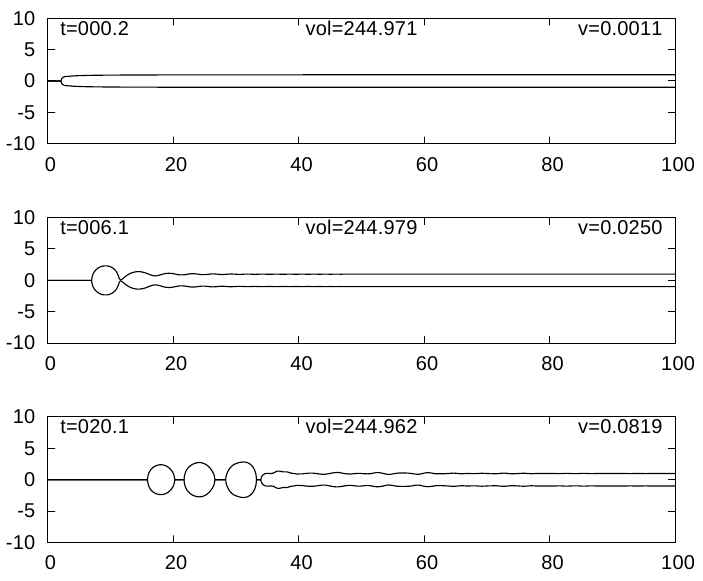
\includegraphics[width=.8\textwidth]{./Slike/mehurcek-rezultat-1}
\caption{"Casovno spreminjanje roba opne med razpadom milnega mehur"cka. Vidno je premikanje fronte in tvorba kapljic s polmerom, ki je dosti ve"cji od debeline opne.~\cite{diploma} }
\label{fig:mehurcek-rez-1}
\end{figure}

Na tej sliki je prikazan le zlom simetrije v smeri potovanja opne. Prikaz je dvodimenzionalen, torej so krogci, ki se odcepljajo od roba, v resnici valji teko"cine. Ti valji razpadejo v kapljice zaradi Rayleighove nestabilnosti, ki je izven obsega tega seminarja. 

Dobljeno hitrost in velikost kapljic lahko preverimo, saj se morata ohranjati tako skupna energija kot tudi celotna prostornina. Skupna prostornina opne in vseh kapljic je izra"cunana na sliki~\ref{fig:mehurcek-rez-1}, med tekom simulacije pa se spremeni za manj kot en promil. Podoben izra"cun lahko naredimo tudi za skupno energijo kapljic in opne.

\subsection{Viskozna opna}
\begin{figure}[h]
  \centering
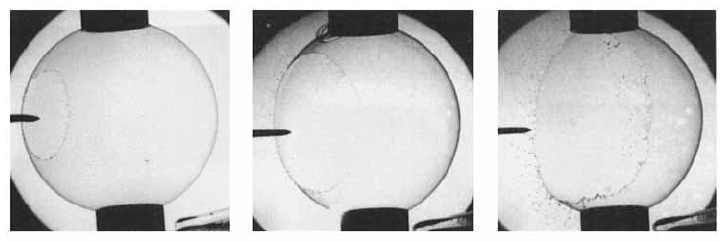
\includegraphics[width=.9\textwidth]{./Slike/meh-vis-1}
\caption{Razpad mehur"cka iz raztopine Teepola z viskoznostjo $\mu = 6$ mPa s.~\cite{pandit}}
\label{fig:mehurcek-viskozni-razpad}
\end{figure}

Opne viskozne teko"cine se v splo"snem obna"sajo druga"ce. Poskusi ka"zejo, da pri dovolj visoki viskoznosti mehur"cek sploh ne razpade v kapljice, ampak se vsa teko"cine nabere na enem mestu. Primer tak"snega razpada je na sliki~\ref{fig:mehurcek-viskozni-razpad}. 

"Ce "zelimo razpad tak"snega mehur"cka modelirati, se spet zate"cemo k numeri"cnim metodam. Re"sujemo Navier-Stokesovo ena"cbo, kjer moramo upo"stevati tudi "clen z viskoznostjo. Ko vse koli"cine pretvorimo v brezdimenzijsko obliko, na gibanje roba opne vpliva le parameter $Z$, ki ga imenujemo Ohnesorgovo "stevilo in predstavlja razmerje med silami zaradi viskoznosti in povr"sinsko napetostjo~\cite{scat}. Podan je kot

\begin{align}
Z &= \mu\sqrt{\frac{\rho}{\sigma a}} 
\end{align}

kjer je $\mu$ viskoznost teko"cine, $\rho$ njena gostota, $\sigma$ povr"sinska napetost, $2a$ pa povpre"cna debelina opne pred razpadom. "Casovno spreminjanje roba pri razli"cnih vrednosti $Z$ je prikazano sa sliki~\ref{fig:mehurcek-rez-vis-1}

\begin{figure}[h]
  \centering
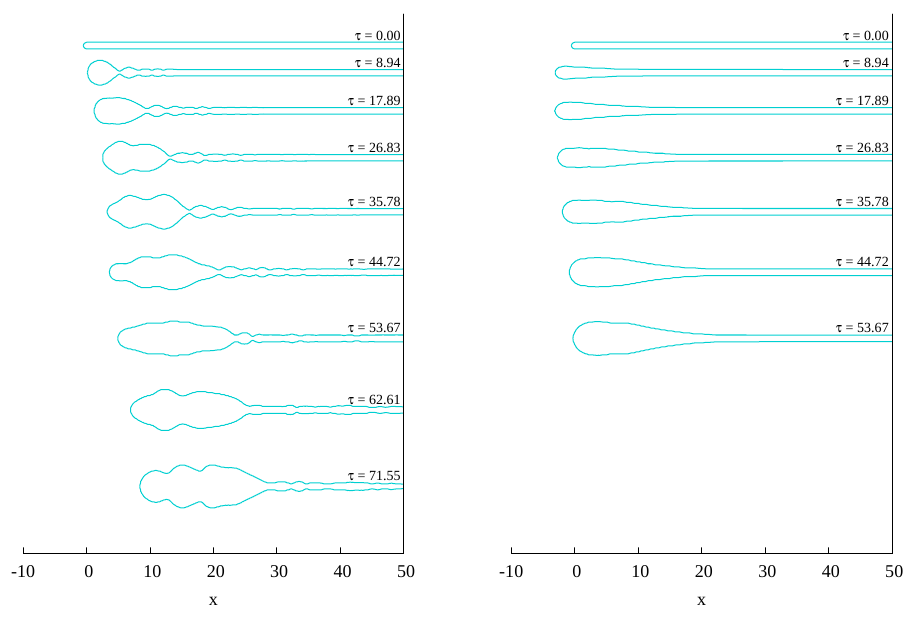
\includegraphics[width=.9\textwidth]{./Slike/scat-rezultat-1}
\caption{Spreminjanje roba opne, ki je dovolj viskozna, da prepre"ci razpad v kapljice.~\cite{scat}
Leva slika prikazuje razvoj roba pri $Z=0,0045$, desna pa pri $Z=4,5$. }
\label{fig:mehurcek-rez-vis-1}
\end{figure}

Obe sliki se kvalitativno razlikujeta od slike~\ref{fig:mehurcek-rez-1}. Valji teko"cine se ne odcepljajo od roba, zato ne pride do razpada v kapljice. Za razpad milni"cnega mehur"cka je viskoznost teko"cine res klju"cnega pomena. 

\section{Kra"ski "zlebi"ci}

"Zlebi"ci so kra"ska tvorba, ki nastane na nagnjenih povr"sinah apnen"castih skal pod vplivom de"zja. So vzporedni "zlebovi v smeri najve"cje strmine. Nastanejo zaradi kislih primesi v de"zevnici, ki po"casi topijo kamnino~\cite{perne,perne-seminar}. Tipi"cno so "siroki nekaj centimetrov. 

\begin{figure}[h]
\centering
 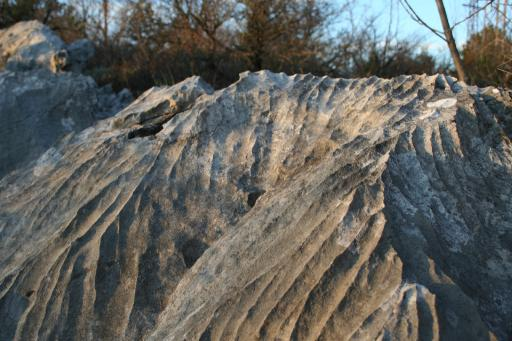
\includegraphics[width=.8\textwidth]{./Slike/Zlebici}
 \caption{"Zlebi"ci na slovenskem Krasu pri Nabre"zini~\cite{wiki:zlebic} }
 \label{fig:zlebici-slika}
\end{figure}

S slike~\ref{fig:zlebici-slika} lahko vidimo, da "zlebi"ci tvorijo podobno periodi"cno strukturo kot teko"cina na sliki~\ref{fig:film-neenakomernost}. Tudi po izvoru sta pojava sorodna: na tistih mestih, kjer "cez "zlebi"c ste"ce ve"c vode, se tudi raztopi ve"c apnenca, torej postane kanal "se globlji in skozenj te"ce "se ve"c vode. Pomembna razlika pa je, da ne opazujemo nestabilnosti v samem toku teko"cine, ampak v obliki podlage. Plast teko"cine tu ni tako tanka, da bi povr"sinska napetost igrala veliko vlogo, je pa "se vedno debelina toka $h$ dosti manj"sa od velikosti pobo"cja, na katerem se tvorijo "zlebi"ci, zato lahko uporabimo lubrikacijski pribli"zek.

Proces tvorbe "zlebi"cev je bolj zapleten kot zgoraj obravnavani primeri. Namesto znane koli"cine vode imamo sedaj neenakomeren de"z, pa tudi pobo"cje ni nujno ravno in homogeno. Ra"cune ote"zi raztapljanje apnenca v vodi, ki je precej razvejan kemijski proces. Navier-Stokesove ena"cbe so zato sklopljene s kemijskimi ena"cbami za raztapljanje. De"z pada v obliki kapljic, ki na mesto padca prinesejo vodo brez raztopljenega apnenca, hkrati pa zmotijo tok teko"cine in na skalno podlago delujejo z neko silo. Vpliva de"znih kapljic ne znamo natan"cno opisati, zato moramo uporabiti poenostavitve. Modeliranje nastanka de"znih "zlebi"cev je zato zelo zahtevno. 

\begin{figure}[h]
 \centering
 \subfigure{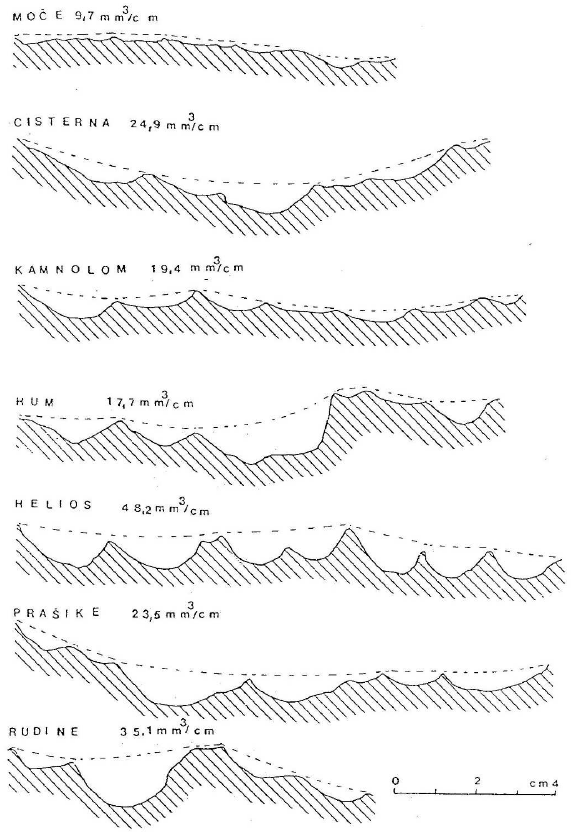
\includegraphics[height=.7\textwidth]{./Slike/zlebici-profil}}
 \subfigure{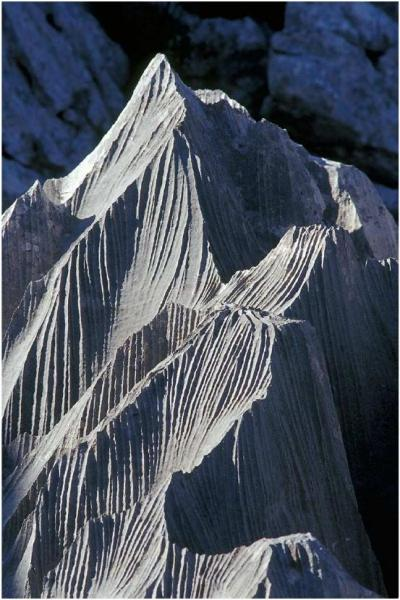
\includegraphics[height=.7\textwidth]{./Slike/zlebici-slika}}
 \caption{Zabele"zeni pre"cni profili "zlebi"cev(levo, \cite{gams}) in skala, prekrita z "zlebi"ci (desno, \cite{perne})}
\end{figure}


Apnenec je slabo topen v vodi, zato je naravni proces nastajanja "zlebi"cev prepo"casen, da bi lahko z njimi izvajali fizikalne eksperimente. Kljub temu pa se ga da pospe"siti, "ce pove"camo koncentracijo kisline v vodi, namesto kamnine pa uporabimo bolje topni mavec. Pomagamo si lahko tudi s "stevilnimi primeri "zlebi"cev najdenih v naravi. Izvedeni poskusi ka"zejo, da "zlebi"ci nastanejo na nagnjeni kamniti povr"sini pri enakomernem de"zju v obliki vodnih kapljic.

Nastajanje "zlebi"cev je neposredna posledica nestabilnosti, le da je motnja v obliki povr"sine, ne pa v profilu toka. "Ce je pobo"cje na za"cetku ravno in se bo majhna motnja s "casom poglabljala, potem bodo s"casoma nastali globlji "zlebi"ci. Matija Perne je v svojem diplomskem delu izvedel simulacijo, s katero je posku"sal pojasniti to nestabilnost. Upo"steval je, da je tok vode po pobo"cju stacionaren, saj je "casovna skala raztapljanja povr"sja mnogo dalj"sa od "casovne skale pojavov v vodnem toku. Zanemaril je tudi vpliv padajo"cih de"znih kapljic po celotnem pobo"cju. Pri teh predpostavkah simulacija da rezultat, pri katerem je pobo"cje stabilno, torej "zlebi"ci s "casom postanejo vedno bolj plitvi. Tak"sen rezultat nasprotuje tako opa"zanjem iz narave kot tudi ekperimentom in je verjetno posledica poenostavitve, kjer zanemarimo vpliv padajo"cega de"zja na raztapljanje kamnine~\cite{perne}. 

\section{Zaklju"cek}

Spoznali smo nekaj primerov pojavov iz vsakdanjega "zivljenja, kjer lahko v toku teko"cine v tanki plasti opazimo nestabilnosti. V seminarju so opisani trije primeri hidrodinamskih sistemov, v katerih poljubno majhna motnja s "casom nara"s"ca, tako da opazimo makroskopsko odstopanje od stacionarnega stanja. Vsi ti sistemi torej ka"zejo neko nestabilnost. 

Pri opisu naravnih pojavov s fizikalnim modelom naletimo na te"zave, saj ne moremo upo"stevati vseh podrobnosti. Nekaterih sploh ne poznamo, druge pa na"crtno zanemarimo, da bo na"s model splo"snej"si in enostavnej"si za re"sevanje. Uporabiti moramo pribli"zke in poenostavitve, kot je na primer lubrikacijski pribli"zek. Zaradi teh poenostavitev izgubimo del informacije o re"sitvi, "se vedno pa lahko napovedujemo stabilnost ali nestabilnost sistema. V nekaterih primerih, kot je tvorba de"znih "zlebi"cih na kra"skem povr"sju, niti ne poznamo vseh detajlov, ki povzro"cijo nestabilnost povr"sja. 

Obravnavani primeri "se zda"lec niso vsi naravni pojavi, kjer se v toku teko"cin pojavljajo nestabilnosti. Opazimo jih lahko pri razpadu teko"cinskih curkov, nastanku morskih valov in turbulentniu tokovih. Zaradi izjemno "sirokega nabora problemov, od katerih nekateri "se niso dobro opisani, "studij stabilnosti v hidrodinamiki ponuja mnogo mo"znosti za raziskovanje. 

\begin{thebibliography}{3}
  \bibitem{drazin} P. G. Drazin, \textit{Introduction to hydrodynamic stability}, Cambridge University Press (2002)
  \bibitem{kondic} L. Kondic, SIAM Review \textbf{45}, 95 (2003)
  \bibitem{slike-mehurcek} \url{http://www.dailymail.co.uk/sciencetech/article-1199149/Super-slow-motion-pictures-soap-bubble-bursting-stunning-detail.html} (23. 1. 2012)
  \bibitem{diploma} S. "Copar, Numeri"cna analiza nestabilnosti na robu teko"cinske opne, Diplomsko delo (2009)
  \bibitem{wiki:zlebic} \href{http://sl.wikipedia.org/wiki/\%C5\%BDlebi\%C4\%8Di}{http://sl.wikipedia.org/wiki/\v Zlebič} (2. 2. 2012)
  \bibitem{gams} I. Gams, Geografija in aktualna vpra"sanja prostorskega razvoja, 127--138 (1989)
  \bibitem{eggers} J. Eggers in E. Villermaux, Rep. Prog. Phys. \textbf{71}, 036601 (2008)
  \bibitem{scat} L. J. Gordillo Zavaleta, Self-similar and travelling wave solutions in surface tension-driven thin planar films, Scientific Computing Advanced Training (2007)
  \bibitem{pandit} A. B. Pandit in J. F. Davidson, J. Fluid Mech. \textbf{212}, 11 (1990)
  \bibitem{perne} M. Perne, Advektivni model topljenja opnenca in nastanek de"znih "zlebi"cev, Diplomsko delo (2007)
  \bibitem{perne-seminar} M. Perne, Physics of karst forms: rillenkarren, Seminar (2006)
\end{thebibliography}


\end{document}
